\documentclass{article}
\usepackage{graphicx} % für das Einfügen von Bildern
\usepackage[ngerman]{babel} % für Spracheinstellung auf Deutsch
\usepackage{parskip} % für Absätze
\usepackage{url} % benötigt für URL in Literaturverzeichnis
\usepackage{amsmath, amssymb} % für mathematische formeln
\usepackage{microtype} % Automatische Optimierung
\usepackage{hyperref} % für hyperlinks
\usepackage[utf8]{inputenc} 
\usepackage[ngerman]{babel} 
\usepackage[T1]{fontenc} 

\title{Abgabe 1 für Computergestützte Methoden}
\author{Gruppe 87\\Jonathan Schäfer(4258298), Felix Schürmann(4296622), Christos Stoupas(2538811) }
\date{Montag, 2. Dezember 2024}

\begin{document}

% Title, Autor und Datum erzeugen
\maketitle

% Inhaltsverzeichnis
\tableofcontents

\newpage

\section{Der zentrale Grenzwertsatz}

Der zentrale Grenzwertsatz (ZGS) ist ein fundamentales Resultat der Wahrscheinlichkeitstheorie, der die Verteilung von Summen unabhängiger, identisch verteilter \textit{(i.i.d.)}  Zufallsvariablen (ZV) beschreibt. Er besagt, dass unter bestimmten Voraussetzungen die Summe einer großen Anzahl solcher ZV annähernd normalverteilt ist, unabhängig von der Verteilung der einzelnen ZV. Dies ist besonders nützlich, da die Normalverteilung gut untersucht und mathematisch handhabbar ist.

\subsection{Aussage}

Sei $X_{1}, X_{2}, \ldots ,X_{n}$ eine Folge von \textit{i.i.d.} ZV mit dem Erwartungswert $\mu = \mathbb{E}(X_{i})$ und der Varianz $\sigma^2 =$ Var$(X_{i})$, wobei $0 < \sigma^2 < \infty$. Dann konvergiert die standardisierte Summe $Z_{n}$ dieser ZV für $n \to \infty$ in Verteilung gegen eine Standardnormalverteilung:\footnote{Der zentrale Grenzwertsatz hat verschiedene Verallgemeinerungen. Eine davon ist der
\textbf{Lindeberg-Feller-Zentrale-Grenzwertsatz }\cite[Seite 328]{Wtheorie}, der schwächere Bedingungen an die Unabhängigkeit und die identische Verteilung der ZV stellt.} 
\begin{equation}
    \label{standardsumme}
    Z_n = \frac{\sum_{i=1}^{n} X_{i}-n\mu}{\sigma\sqrt{n}} \xrightarrow{d} \mathcal{N}(0,1).
\end{equation}
Das bedeutet, dass für große $n$ die Summe der ZV näherungsweise normalverteilt ist mit Erwartungswert $n\mu$ und Varianz $n\sigma^2$:
\begin{equation}
    \label{normalverteilteZV}
    \sum_{i=1}^{n} X_{i} \sim \mathcal{N}(n\mu,n\sigma^2).
\end{equation}

\subsection{Erklärung der Standardisierung}

Um die Summe der ZV in eine Standardnormalverteilung zu transformieren, subtrahiert man den Erwartungswert $n\mu$ und teilt durch die Standardabweichung $\sigma\sqrt{n}$. Dies führt zu der obigen Formel \eqref{standardsumme}. Die Darstellung \eqref{normalverteilteZV} ist für $n\to\infty$ nicht wohldefiniert.

\subsection{Anwendung}

Der ZGS wird in vielen Bereichen der Statistik und der Wahrscheinlichkeitstheorie angewendet. Typische Beispiele sind:

\begin{itemize}
    \item \textbf{Würfelspiel}: \\
    Seien $X_{i}$, $i = 1,\ldots,n$, \textit{(i.i.d.)} Zufallsvariablen (ZV) mit $P(X_{i} = k) = \frac{1}{6}$ für $k \in \{1,2,3,4,5,6\}$. \\Es gilt $\mu = \mathbb{E}(X_{i}) = 3,5$ und $\sigma^2 = \frac{35}{12} \approx 2,92$. Dann konvergiert die standardisierte Summe $Z_{n}$ der $X_{i}$ für $n \to \infty$ gegen die Standardnormalverteilung und es gilt:
    \begin{equation}
        P(Z_{n} \le x) \approx \phi(x) \notag
    \end{equation}
    wobei $\phi$ die Verteilungsfunktion der Standardnormalverteilung ist. \\Sei nun $x=370$ und $n=100$, wir wollen also berechnen, wie wahrscheinlich es ist, dass insgesamt bei 100 Würfen die aufsummierte Augenzahl 370 oder weniger beträgt.
    
    \begin{equation}
        Z_{100} = \frac{\sum_{i=1}^{100} X_{i} - n\mu}{\sigma\sqrt{n}} = \frac{370 - 350}{17,08} \approx 1,17 \notag 
    \end{equation}
    
    \begin{equation}
        \phi(1,17) \approx 0,8790 \notag
    \end{equation}
    
    Das bedeutet, die Wahrscheinlichkeit, dass die Summe aller einzelnen Würfe 370 oder weniger beträgt, ist 87,9 \%.
    
    \item \textbf{LED-Produktion}:\\
    Die Wahrscheinlichkeit für die Produktion einer fehlerhaften LED sei $p$. Wie groß ist die Wahrscheinlichkeit, bei $n$ LEDs höchstens $k$ defekte zu haben?
    Modellierung als Bernoulli-Experiment:\\
    Jeder LED entspricht eine Zufallsvariable $X_{i}$ mit Wert $X_{i}=1$ und Wahrscheinlichkeit $P(X_{i}=1)=p$, falls sie defekt ist, und den Wert $X_{i} = 0$ mit Wahrscheinlichkeit $P(X_{i} = 0 ) = 1-p$, wenn sie in Ordnung ist. Die standardisierte Anzahl defekter LEDs unter $n$ Stück ist $Z_{n}$.\\
    Gesucht ist $P(Z_{n} \ge x)$. Dann gilt nach dem zentralen Grenzwertsatz:
    \begin{equation}
        P(Z_{n} \ge x) \approx 1-\phi(x) \notag 
    \end{equation}
    Sei nun $p=0,01$, $n=1000$ und $x=15$. Wir suchen also die Wahrscheinlichkeit, dass unter 1000 LEDs mehr als 15 defekt sind. Dann gilt:
    
    \begin{equation}
        Z_{1000} = \frac{\sum_{i=1}^{1000} X_{i} - n\mu}{\sigma\sqrt{n}} = \frac{15 - 1000\cdot0,01}{\sqrt{0,01 \cdot 0,99 \cdot 1000}} = \frac{15 - 10}{3,146} \approx 1,59 \notag 
    \end{equation}
    
    \begin{equation}
        1-\phi(1,59) \approx 1-0,9441=0,0559 \notag
    \end{equation}
    
    Das heißt, die Wahrscheinlichkeit, dass mehr als 15 LEDs kaputt sind, ist gerade 5,59 \%.
\end{itemize}


\newpage
\section{Bearbeitung zur Aufgabe 1}
\subsection{Untersuchung des für die Gruppe relevanten Teils der Daten}

In dieser Arbeit analysieren wir unsere Erkenntnisse und Lösungsansätze bezüglich des gruppeneigenen Datenteils. Der untersuchte Datenteil betrifft die Station \textit{W 42 St \& 8 Ave}. Diese Station ist ein spezifischer Wert des Attributes \textit{station} und umfasst die Zeilen 31.343 bis 31.707, folglich 364 Zeilen, des gesamten Datensatzes, der insgesamt 36.440 Zeilen enthält. Die Spaltenreihenfolge des Datensatzes lautet: 
\textit{group}, \textit{station}, \textit{date}, \textit{day\_of\_year}, \textit{day\_of\_week}, \textit{month\_of\_year}, \textit{precipitation}, \textit{windspeed},  \textit{min\_temperature}, \textit{average\_temperature}, \textit{max\_temperature} und \textit{count}. Das Format des Datums entspricht der DIN 1355-1 Schreibweise und deckt den Zeitraum vom \textit{01.01.2023} bis zum \textit{31.12.2023} ab. Der niedrigste Wert des Attributes \textit{date} ist somit der \textit{01.01.2023}, während der höchste Wert der \textit{31.12.2023} ist. 

Das Attribut \textit{count} scheint die Anzahl der an einem Tag erfolgten Fahrradverleihungen zu repräsentieren. Der niedrigste Wert ist \textit{-1}, während der höchste \textit{394} beträgt. Es gibt jedoch auch leere Einträge in dieser Spalte. Die Werte für \textit{wind\_speed} reichen von \textit{-1} bis \textit{25,72}. Die Spalte \textit{precipitation} beschreibt die Niederschlagsmenge und der höchste beträgt \textit{8,05}. Dieser kann in $mm$ oder $l/m^2$ berechnet sein. Die Angaben würden sich dabei aber nicht unterscheiden\footnote{Informationen zu den Einheiten und Messmethoden von Niederschlagsmengen\cite{tfa_niederschlag}}. Das Attribut \textit{min\_temperature} zeigt Werte zwischen \textit{-1} und \textit{76}, während \textit{max\_temperature} Werte von \textit{-1} bis \textit{93} und \textit{average\_temperature} Werte von \textit{-1} bis \textit{83} umfasst. Die Temperatur wird in Fahrenheit gemessen. Zu erkennen ist außerdem, dass sich die Wetterdaten an spezifischen Tagen nicht von Station zu Station unterscheiden.

Eine Korrelation zwischen den Temperaturen und den Jahreszeiten ist erkennbar: Die Temperaturen steigen und fallen entsprechend der Saison. Besonders auffällig sind die NA-Werte in mehreren Spalten, die aus der zugrundeliegenden CSV-Datei übernommen wurden.
Außerdem gibt es für jede Zeile des Wetters betreffende Daten mindestens einen Eintrag von -1. Dabei ist zu vermerken, dass sich die Wetterdaten doppeln, da für jede Station, jedes Datum jeweils einmal vorkommt und die Wetterdaten hier immer identisch sind. Daher sind die Werte von -1, auch wenn nicht direkt unlogisch für die Temperaturdaten, dennoch als fehlerhafte Daten zu klassifizieren.

\subsection{Bereinigung der Daten}

Für die Bereinigung des Datensatzes zum Import in eine Tabellenkalkulation wurde \textbf{Google Colab} in Verbindung mit Python verwendet. Der folgende Python-Code wurde eingesetzt, um die Daten zu verarbeiten:\\ 


\begin{verbatim}
import pandas as pd
# Laden des Datensatzes
df = pd.read_csv('/content/bike_sharing_data_(with_NAs).csv')

# Filtern der Daten für eine spezifische Gruppe
filtered_df = df[df['group'] == 87]
filtered_df = filtered_df.drop('group', axis=1)

# Entfernen der Zeilen mit NA-Werten
cleaned_df = filtered_df.dropna()

# Umwandlung der Temperaturspalten, der Zählspalte und der Spalten für Tag,
Woche und Monat in Ganzzahlen
cleaned_df['min_temperature'] = cleaned_df['min_temperature'].astype(int)
cleaned_df['average_temperature'] = cleaned_df['average_temperature'].astype(int)
cleaned_df['max_temperature'] = cleaned_df['max_temperature'].astype(int)
cleaned_df['count'] = cleaned_df['count'].astype(int)
cleaned_df['day_of_year'] = cleaned_df['day_of_year'].astype(int)
cleaned_df['day_of_week'] = cleaned_df['day_of_week'].astype(int)
cleaned_df['month_of_year'] = cleaned_df['month_of_year'].astype(int)

# Speichern der bereinigten Daten in einer neuen CSV-Datei
cleaned_df.to_csv('cleaned_data.csv', index=False)

# Ermöglichen des Downloads der bereinigten Datei
from google.colab import files
files.download('cleaned_data.csv')
\end{verbatim}


Der Grund für die Bereinigung war, dass der ursprüngliche Datensatz mehrere NA-Werte (Not Available) enthielt und wir nur die gruppenspezifischen Einträge betrachten wollten, ohne die Filterfunktion der Tabellenkalkulation zu verwenden. Dadurch ließ sich im Nachgang ebenfalls die Berechnung der Temperatur dynamischer gestalten. Die bereinigten Daten wurden abschließend in einer neuen CSV-Datei mit dem Namen \textit{cleaned\_data.csv} gespeichert und zur weiteren Verarbeitung heruntergeladen. 


\subsection{Import der CSV-Datei in eine Tabellenkalkulation}

Im folgenden Abschnitt wird erläutert, wie die CSV-Datei in eine Tabellenkalkulation importiert wurde, in unserem Fall war es Microsoft \textbf{Excel}. Es wurde in \textbf{Excel} eine leere Arbeitsmappe geöffnet. Unter dem Reiter \textit{Daten} wurde die Option \textit{Daten abrufen}, gefolgt von \textit{aus Datei} und schließlich \textit{aus Text/CSV} ausgewählt. Danach wurde die heruntergeladene Datei im entsprechenden Verzeichnis ausgewählt. 

Daraufhin öffnete sich der Excel-Assistent und es wurde hier als Trennzeichen \textit{Komma} ausgewählt.
Außerdem mussten die Daten noch transformiert werden. Dazu wurde auf \textit{Daten transformieren} geklickt und in der Formel für \textit{„Geänderter Typ“} die Werte für \textit{{"precipitation", Int64.Type}} und \textit{{"windspeed", Int64.Type}} herausgelöscht. Dieser Schritt war notwendig, um sicherzustellen, dass die Daten in den richtigen Datentyp umgewandelt wurden, bevor mit der weiteren Verarbeitung fortgefahren werden konnte. Anschließend wurde auf \textit{Laden} geklickt, um die Daten in die Arbeitsmappe zu importieren. Nach diesen Schritten war die CSV-Datei erfolgreich als Tabelle in \textbf{Excel} geöffnet und für die weitere Bearbeitung bereit.

\subsection{Berechnung der höchsten mittleren Temperatur per Tabellenkalkulation}

Zur Berechnung der höchsten mittleren Temperatur der gruppeneigenen Station in Grad Celsius wurden Formeln in \textbf{Excel} verwendet. Zunächst wählten wir eine leere Zeile in \textbf{Excel} aus und verwendeten die folgende Formel, um die höchste mittlere Temperatur in Celsius zu berechnen\footnote{Metric Conversion of Fahrenheit\cite{metric_conversions_fahrenheit}}:
\[
=(MAX(I:I)-32) \times \left(\frac{5}{9}\right)
\]
Diese Formel berechnete die Temperatur in Celsius, indem sie den höchsten Wert der Spalte \textit{I} (welcher die durchschnittlichen Temperaturen in Fahrenheit enthält) um 32 reduzierte und anschließend mit dem Faktor \(\frac{5}{9}\) multiplizierte. Das Ergebnis dieser Berechnung war eine Temperatur von $28.33^\circ\text{C}$. 
\begin{figure}[ht] 
    \centering
    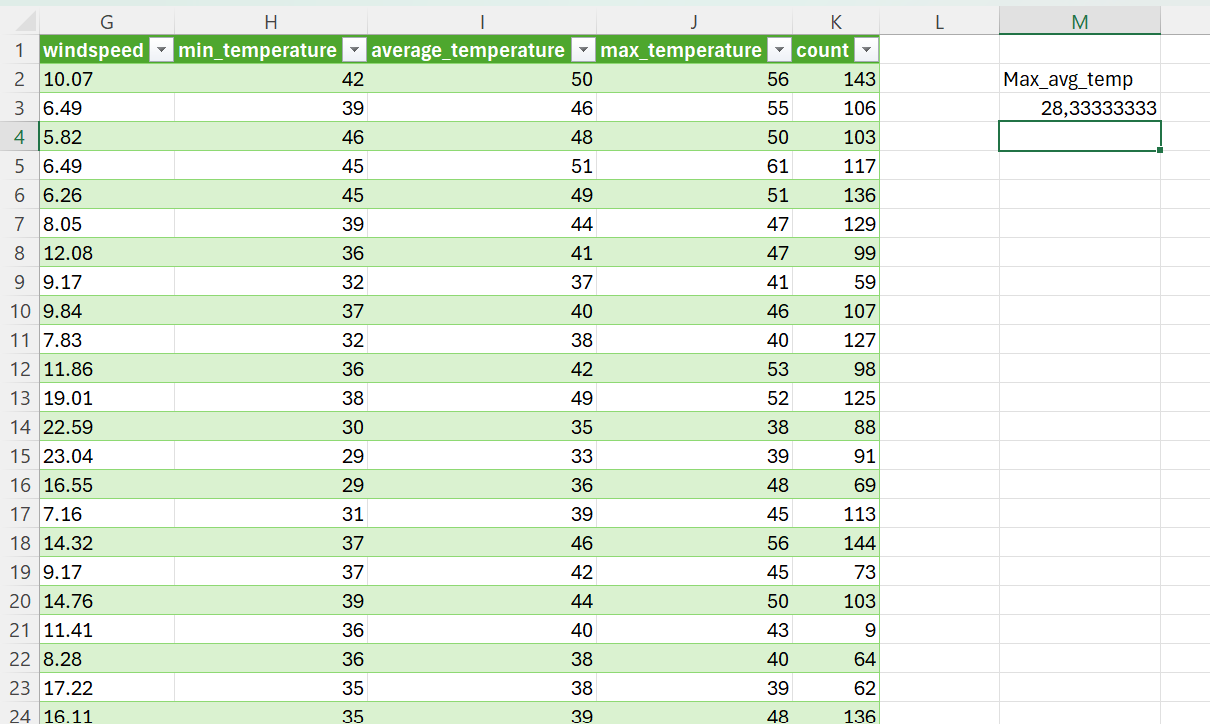
\includegraphics[width = \textwidth]{Screenshot 2024-11-25 111035.png}
    \caption{Berechnung in der Tabellenkalkulation}
    \label{fig:dax}
\end{figure}
\newpage
\subsection{Entwerfen eines Datenbank Schemas}

Im Folgenden wird das entwickelte Datenbankschema beschrieben, das auf den gruppenspezifischen Stationen und Wetterdaten basiert. Dabei werden auch die Anforderungen der ersten und zweiten Normalform berücksichtigt.

\textbf{Datenbank Schemas}

\begin{itemize}
  \item \textbf{Station} (ID\#, Name)
  \item \textbf{Wetter} (ID\#, precipitation, windspeed, min\_temperature, average\_temperature, max\_temperature)
  \item \textbf{Verleih} (ID\#, date, StationID\#, WetterID\#, count)
\end{itemize}

\subsection*{1. Normalform}

Die erste Normalform (1NF) verlangt, dass alle Attribute einer Tabelle atomar sind. Das bedeutet, dass jedes Attribut nur einen einzelnen Wert pro Zeile enthalten darf. In unserem Fall wurden alle Tabellen so strukturiert, dass jedes Attribut einen einzelnen, atomaren Wert enthält, welcher die 1NF erfüllt.
Das entwickelte Schema besteht aus drei Tabellen:

\begin{itemize}
    \item In der Tabelle \textbf{Station} sind die Attribute \textit{ID\#} (eine eindeutige Identifikationsnummer) und \textit{Name} (der Name der Station) enthalten.
    \item Die Tabelle \textbf{Wetter} enthält die Wetterdaten für einen spezifischen Tag. Die Attribute wie \textit{precipitation}, \textit{windspeed}, \textit{min\_temperature}, \textit{average\_temperature} und \textit{max\_temperature} speichern die entsprechenden Wetterdaten.
    \item Die Tabelle \textbf{Verleih} speichert die Verleihdaten, einschließlich der Verleihanzahl und einer Referenz zu den Stationen und Wetterdaten. Das Datum wird in der Tabelle \textit{Verleih} gespeichert, um jeden Verleihvorgang einem bestimmten Zeitpunkt zuzuordnen.
\end{itemize}


\subsection*{Hinweis zur Verwendung von Datumsangaben}

In Bezug auf die Angaben des Datums wird das Datum in der Tabelle \textbf{Verleih} gespeichert, da jeder Verleihvorgang einem bestimmten Zeitpunkt zugeordnet wird. In \textbf{SQL} kann die Funktion \texttt{WEEKDAY()}\footnote{Karriere Tutor, SQL Befehle\cite{karrieretutor_sql}} verwendet werden, um den Wochentag basierend auf dem Datum zu ermitteln. Alle anderen relevanten Informationen wie der Monat oder das Jahr können ebenfalls direkt aus dem Datum abgelesen oder abgeleitet werden. Daher werden Informationen über \textit{month\_of\_year} oder \textit{day\_of\_weak} nicht benötigt. Theoretisch würde auch das Feld  \textit{day\_of\_year} nicht benötigt. Allerdings wird dieses im späteren Verlauf genutzt, um in der Tabelle \textbf{Wetter} den primären Schlüssel zu setzen.

\subsection*{2. Normalform}

Die zweite Normalform (2NF) besagt, dass das Schema in mehrere Tabellen aufgeteilt werden soll und es Fremdschlüsselbeziehungen mit passenden Abhängigkeiten gibt.
So wurden die Werte aus der CSV-Datei in 3 Tabellen aufgeteilt, damit sie logisch eigene Entitäten darstellen.


Im entwickelten Datenbankschema sind die Tabellen so gestaltet, dass sie die 2NF erfüllen:
\begin{itemize}
    \item In der Tabelle \textbf{Station} ist das Attribut \textit{ID\#} der Primärschlüssel und das Attribut \textit{Name} hängt vollständig von diesem Schlüssel ab.
    \item In der Tabelle \textbf{Wetter} wird die \textit{WetterID\#} als Primärschlüssel verwendet und alle anderen Attribute (z. B. \textit{precipitation}, \textit{windspeed}) hängen vollständig von dieser ID ab.
    \item  In der Tabelle \textbf{Verleih} sind \textit{StationenID\#} und \textit{WetterID\#} als Fremdschlüssel angegeben, die auf die entsprechenden Datensätze in den Tabellen \textbf{Station} und \textbf{Wetter} verweisen. Das \textit{Datum} wird in der Tabelle \textbf{Verleih} gespeichert, da es den Verleihvorgang zu einem bestimmten Zeitpunkt zuordnet. Alle anderen Attribute hängen vollständig vom Primärschlüssel ab.
\end{itemize}




Dieses Schema stellt sicher, dass alle Daten in einer formalen, relationalen Struktur vorliegen, die effizient abgerufen und bearbeitet werden kann.

\subsection{Übersetzung des Schemas in SQL}

Im folgenden Verlauf übersetzen wir die Schemata in das Programm \textbf{SQL}. Zuerst öffnen wir den \textbf{SQLite Editor}.\\Im nächsten Schritt erstellen wir die Tabellen basierend auf dem erstellten Schema. Wir legen die Tabellen im oben benannten Muster nach demselben Vorgehen über folgende \textbf{SQL} Befehle an:
\begin{verbatim}
CREATE TABLE stationen (
    id INTEGER PRIMARY KEY,
    name TEXT);
\end{verbatim}

Für die zweite Tabelle, \textbf{Wetter}, verwenden wir den folgenden SQL-Befehl:
\begin{verbatim}
CREATE TABLE wetter (
    id INTEGER PRIMARY KEY,
    precipitation DECIMAL,
    windspeed DECIMAL,
    min_temperature INTEGER,
    max_temperature INTEGER,
    average_temperature INTEGER);
\end{verbatim}
\newpage
Schließlich erstellen wir die Tabelle \textbf{Verleih} mit diesem Befehl:
\begin{verbatim}
CREATE TABLE verleih (
    id INTEGER PRIMARY KEY,
    wetterid INTEGER,
    stationenid INTEGER,
    date DATE,
    count INTEGER,
    FOREIGN KEY(wetterid) REFERENCES wetter(id),
    FOREIGN KEY(stationenid) REFERENCES stationen(id));
\end{verbatim}

\begin{figure}[ht] 
    \centering
    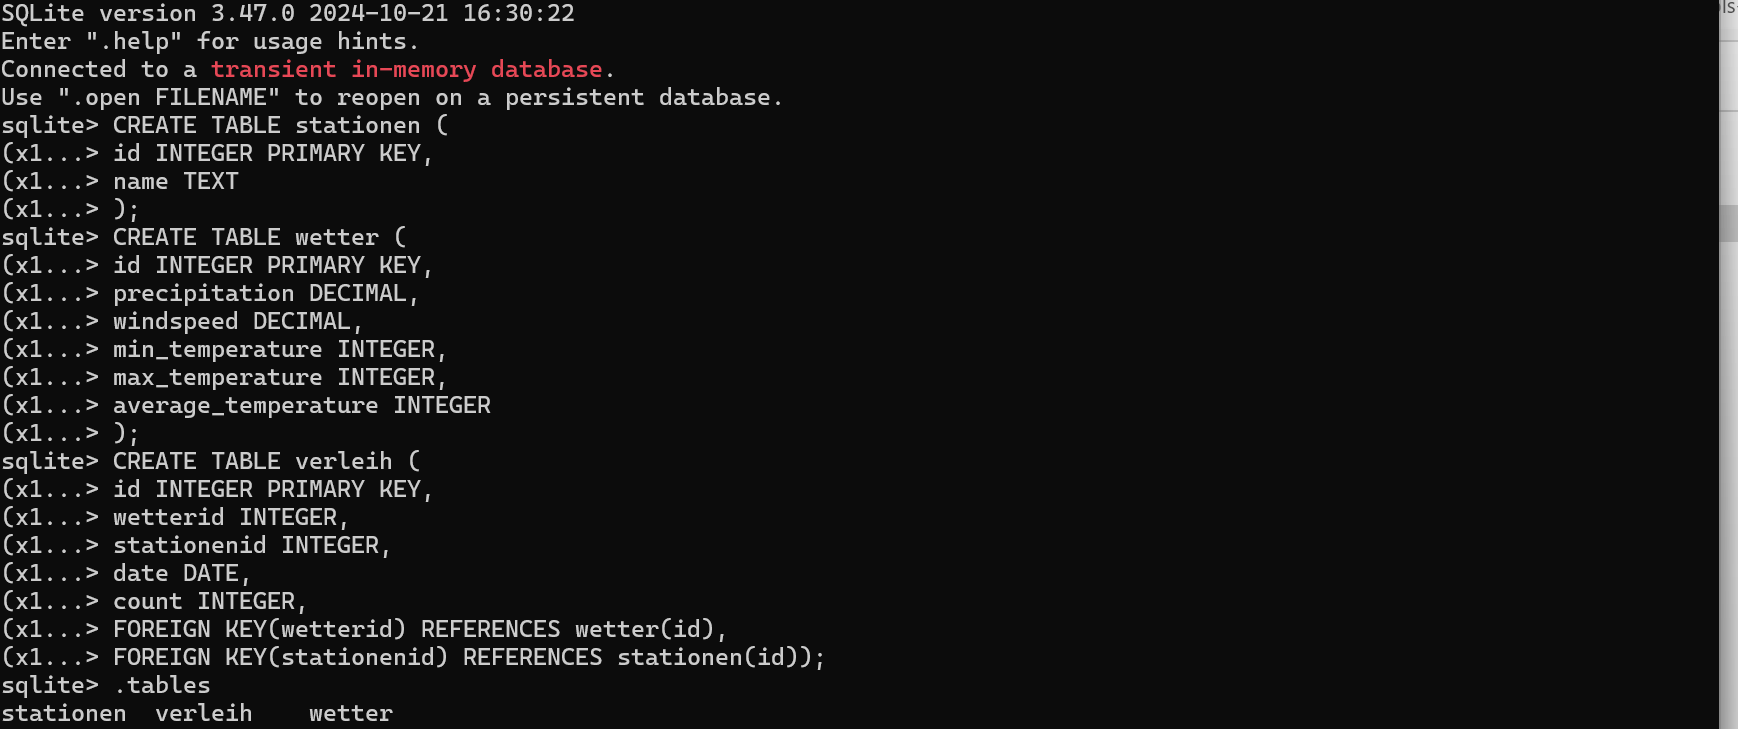
\includegraphics[width = \textwidth]{Screenshot 2024-11-24 183300.png}
    \caption{Erstellung der Tabellen}
    \label{fig:dax}
\end{figure}

Die Datentypen \texttt{INTEGER}, \texttt{DECIMAL}, \texttt{DATE} und \texttt{TEXT} wurden gewählt, um den jeweiligen Attributwerten zugerechnet zu werden. Die \texttt{INTEGER}-Werte repräsentieren die IDs, die als Primärschlüssel dienen. Die \texttt{DECIMAL}-Werte wurden für \texttt{precipitation} und \texttt{windspeed} gewählt, um Dezimalstellen korrekt abzubilden. Das \texttt{DATE}-Format für das \texttt{date}-Attribut sorgt dafür, dass die Angaben des Datums richtig gespeichert werden. Zudem wurden in der Tabelle \textbf{Verleih} die Fremdschlüssel \texttt{wetterid} und \texttt{stationenid} definiert, die auf die entsprechenden Primärschlüssel in den Tabellen \textbf{Wetter} und \textbf{Stationen} verweisen, wodurch die referenzielle Integrität gewährleistet ist.

\subsection{Aufbereiten der Datensätze und importieren in die Tabellen}

Um die Daten korrekt in die Tabellen zu importieren, mussten einige Anpassungen vorgenommen werden. Hierzu wurde, wie bereits zuvor, ein Python-Skript genutzt, welches auf \textbf{Google Colab} durchgeführt wurde. 

Zunächst wurden die Daten in die Umgebung importiert. Da zusätzlich zu den Zeilen mit leeren Werten Werte von -1 existieren, wurden diese untersucht. Diese Werte sind im Kontext allerdings für alle Felder außer den Temperaturangaben nicht sinnvoll. Bei genauer Betrachtung konnte festgestellt werden, dass sich die Temperaturangaben doppeln. Diese sind für alle Stationen über den Verlauf des Jahres gleich, und alle Felder, welche eine -1 enthalten, sind für die restlichen Tage mit einem anderen Wert befüllt. Daher konnte davon ausgegangen werden, dass es sich hierbei ebenfalls um fehlerhafte Daten handelt, und diese wurden entfernt. 

Außerdem konnten die Spalten \texttt{group}, \texttt{day\_of\_week} und \texttt{month\_of\_year} ebenfalls entfernt werden, da diese nicht atomar sind, wie bereits zuvor beschrieben. Das Feld \texttt{day\_of\_year} jedoch wurde behalten, da dieses zur Verwendung als Primary Key in der Tabelle \textbf{Wetter} genutzt werden kann (Werte von 1 bis 365). 

Daraufhin mussten zwei weitere Spalten hinzugefügt werden, welche die Primary Keys für die Tabellen \textbf{Verleih} und \textbf{Stationen} darstellen. Dies wurde umgesetzt, indem anhand der relevanten Spalten jeweils nur die einzigartigen Werte genommen und ab 1 aufgezählt wurden. 

Zuletzt mussten die Werte der Tabellen aufgrund der Pandas-Logik wieder in ihre ursprünglichen Datentypen transformiert werden, bevor die Dateien heruntergeladen werden konnten.

\subsection*{Python-Code für die Datenaufbereitung}

\begin{verbatim}
import pandas as pd
from google.colab import files

# Laden des Datensatzes
df = pd.read_csv('/content/bike_sharing_data_(with_NAs).csv')
# -1 stellt fehlerhafte Daten dar
#Eird daher zu einem NA Wert verändert um es hinterher zu entfernen
df.replace(["", -1], pd.NA, inplace=True)
# Entfernen von nicht atomaren Werten
df = df.drop(['group', 'day_of_week', 'month_of_year'], axis=1)
# Entfernen fehlerhafter Daten
df = df.dropna(how='any', axis=0)
# Erstellen eines Primary Keys für die Verleih Tabelle
#Und der Stationen Tabelle anhand des Stationennamen
df['verleihid'] = pd.factorize(list(zip(df['date'], 
    df['station'])))[0]+1
df['stationenid'] = pd.factorize(df['station'])[0] + 1
# Transformieren der Datentypen zu korrektem Typ
df['day_of_year'] = df['day_of_year'].astype(int)
df['min_temperature'] = df['min_temperature'].astype(int)
df['average_temperature'] = df['average_temperature'].astype(int)
df['max_temperature'] = df['max_temperature'].astype(int)
df['count'] = df['count'].astype(int)



# Erstellen der für den Import benötigten Tabellen
wetter_tabelle = df[['day_of_year', 'precipitation',
    'windspeed', 'min_temperature', 
    'max_temperature', 'average_temperature']]
wetter_tabelle = wetter_tabelle.drop_duplicates()
stationen_tabelle = df[['stationenid', 'station']]
stationen_tabelle = stationen_tabelle.drop_duplicates()
verleih_tabelle = df[['verleihid', 'day_of_year', 
    'stationenid', 'date', 'count']]
verleih_tabelle = verleih_tabelle.drop_duplicates()

# Herunterladen der Tabellen als CSV Datei
wetter_tabelle.to_csv('/content/wetter_tabelle.csv', index=False)
stationen_tabelle.to_csv('/content/stationen_tabelle.csv', index=False)
verleih_tabelle.to_csv('/content/verleih_tabelle.csv', index=False)

files.download('/content/wetter_tabelle.csv')
files.download('/content/stationen_tabelle.csv')
files.download('/content/verleih_tabelle.csv')
\end{verbatim}

\subsection{Importieren der Daten in das SQL Schema}

\subsection*{Import der Daten in SQLite}

Beim Import der Daten in die SQLite-Datenbank wurde der folgenden Anleitung aus dem SQLite-Tutorial gefolgt\footnote{Anleitung basiert auf dem SQL-Tutorial von W3Schools\cite{w3schools_sql}}: 

\begin{itemize}
    \item \texttt{.mode csv}: 
    Ändert den Modus auf CSV
    \item \texttt{.separator ","}:
    Wird genutzt um den Separator auf \textit{Komma} zusetzen, damit die Datei korrekt ausgelesen werden kann
    \item \texttt{.import --skip 1 FILEPATH TABLENAME}:
    Wird für den Import der Dateien genutzt, wobei \texttt{--skip 1} dafür steht, dass die erste Zeile der CSV-Datei übersprungen wird, da diese die Spaltenüberschriften enthält.
\end{itemize}


Nach dem Import wurde überprüft, ob die Daten korrekt in den Tabellen abgelegt wurden und ob Werte vorhanden sind. Dies wurde durch den Befehl \texttt{SELECT * FROM TABLENAME} durchgeführt. Um die Darstellung der Ergebnisse zu verbessern, wurde der Befehl \texttt{.mode column} und \texttt{.headers on} verwendet, um die Ausgabe in einer tabellarischen Form mit Spaltenüberschriften anzuzeigen.
\begin{figure}[ht] 
    \centering
    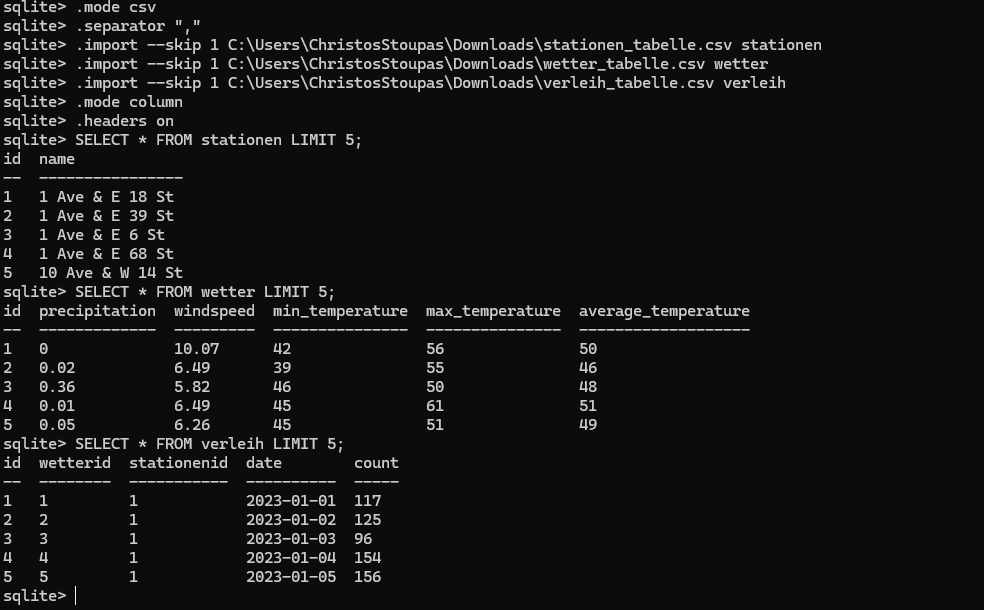
\includegraphics[width = \textwidth]{Screenshot 2024-11-24 201336.png}
    \caption{Import der CSV Dateien und Überprüfung}
    \label{fig:dax}
\end{figure}

\newpage
\subsection{Berechnung der höchsten mittleren Temperatur per SQL Abfrage}

Zur Berechnung der höchsten mittleren Temperatur wurde folgendes SQL-Statement verwendet:

\begin{verbatim}
SELECT ((MAX(CAST(w.average_temperature AS REAL)) - 32) * 5.0 / 9.0) 
AS max_average_temperature
FROM wetter w
JOIN verleih v ON w.id = v.wetterid
WHERE v.stationenid = 87;
\end{verbatim}

\textbf{Erklärung des SQL-Statements:}

Im SQL-Statement wählen wir zunächst mit dem \texttt{SELECT}-Befehl die höchste durchschnittliche Temperatur aus der Tabelle aus. Dabei verwenden wir die Funktion \texttt{MAX}, um den maximalen Wert aus der Spalte \texttt{average\_temperature} zu ermitteln. Da die Temperaturwerte in der Tabelle jedoch als Fahrenheit-Werte gespeichert sind, ist es notwendig, diese in den Datentyp \texttt{REAL} umzuwandeln, damit wir die mathematische Berechnung korrekt durchführen können. Dies geschieht durch die Verwendung der \texttt{CAST}-Funktion, die den Wert von Fahrenheit in einen Datentyp umwandelt, der Dezimalzahlen (Realwerte) unterstützen kann.

Das Ergebnis dieser Berechnung wird mit dem Alias \texttt{max\_average\_temperature} versehen, um es besser verständlich zu machen und im Abfrageergebnis eindeutig zu kennzeichnen.

Die Daten, die für diese Berechnung verwendet werden, stammen aus der Tabelle \textbf{Wetter}, die hier mit dem Alias \texttt{w} bezeichnet wird. Um auf die relevanten Wetterdaten zugreifen zu können, erfolgt ein \texttt{JOIN} mit der Tabelle \textbf{Verleih} (Alias \texttt{v}). Der \texttt{JOIN} wird durch die Bedingung \texttt{w.id = v.wetterid} durchgeführt, wodurch die Daten aus beiden Tabellen miteinander verknüpft werden. Dies stellt sicher, dass die Wetterdaten mit den Verleihdaten kombiniert werden, um die Berechnung der höchsten Temperatur für eine bestimmte Station durchzuführen.

Schließlich wird durch den \texttt{WHERE}-Befehl festgelegt, dass nur der Datensatz für die Station mit der ID 87 berücksichtigt wird. Diese Einschränkung sorgt dafür, dass die Berechnung der höchsten mittleren Temperatur nur für diese spezifische Station durchgeführt wird und nicht für alle Stationen in der Datenbank.

Das Ergebnis kam analog zum Ergebnis in der Tabellenkalkulation heraus: $28.33^\circ\text{C}$.


\begin{figure}[ht] 
    \centering
    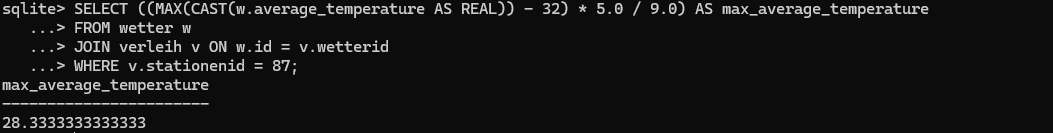
\includegraphics[width = \textwidth]{Screenshot 2024-11-24 202033.png}
    \caption{Berechnung der Temperatur}
    \label{fig:dax}
\end{figure}


\newpage
\bibliographystyle{unsrt}
\bibliography{reference}

\end{document}
